\section{Apprentissage profond supervisé}

\subsection{L'IA "maison"}
	
	\begin{frame}{Un peu de théorie}
		\begin{block}{Ici}
            % TODO : A compléter
	    \end{block}
	\end{frame}
	
	\begin{frame}{Amélioration et Entraînement}
	    \begin{figure}
	        \centering
	        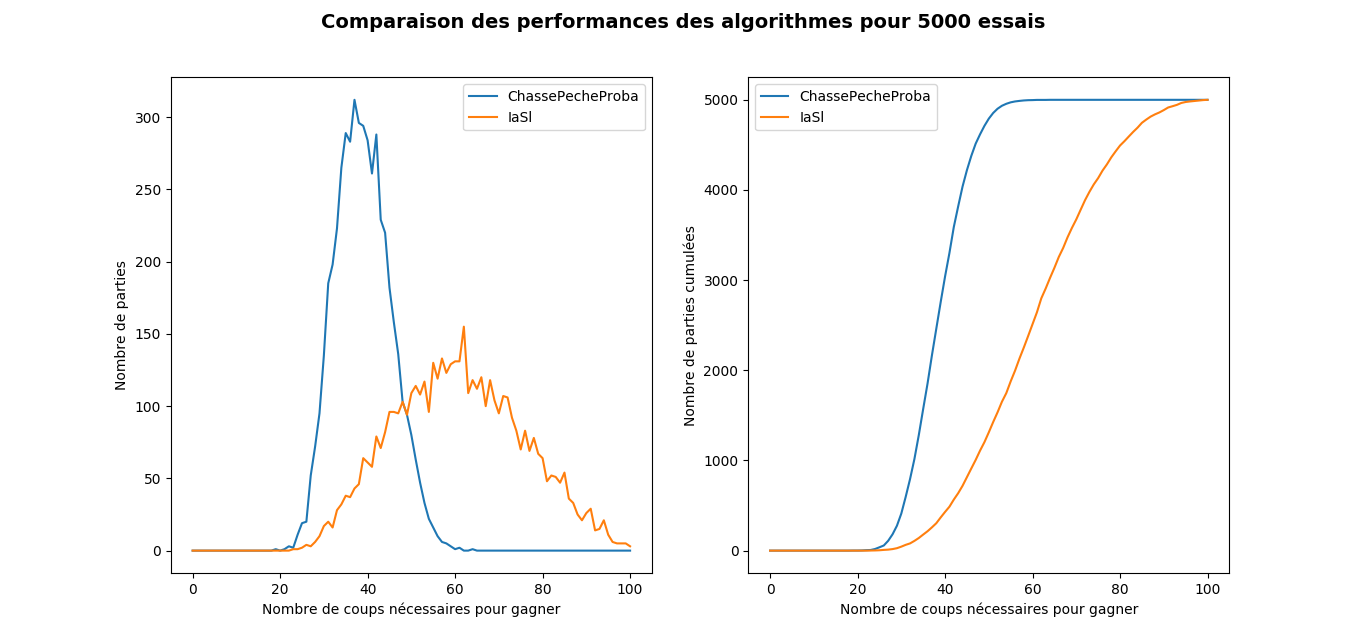
\includegraphics[width=.95\linewidth]{images/perfiasl1.png}
	        \caption*{Performance IA V1}
	        \label{fig:perfiasl1}
	    \end{figure}{}
	\end{frame}{}
	
	\begin{frame}{Amélioration et Entraînement}
	    \begin{figure}
	        \centering
	        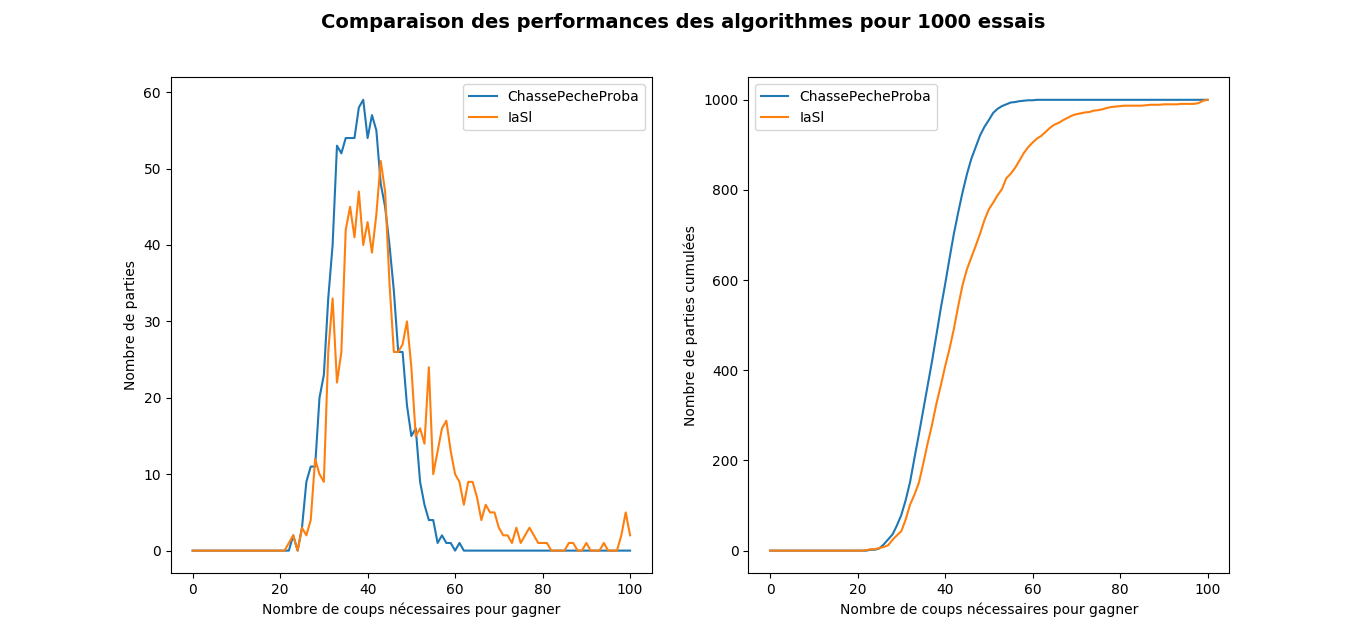
\includegraphics[width=.95\linewidth]{images/perfiasl2.png}
	        \caption*{Performance IA V2 (quelques minutes d'entraînement)}
	        \label{fig:perfiasl2}
	    \end{figure}{}
	\end{frame}{}
	
	\begin{frame}{Amélioration et Entraînement}
	    \begin{figure}
	        \centering
	        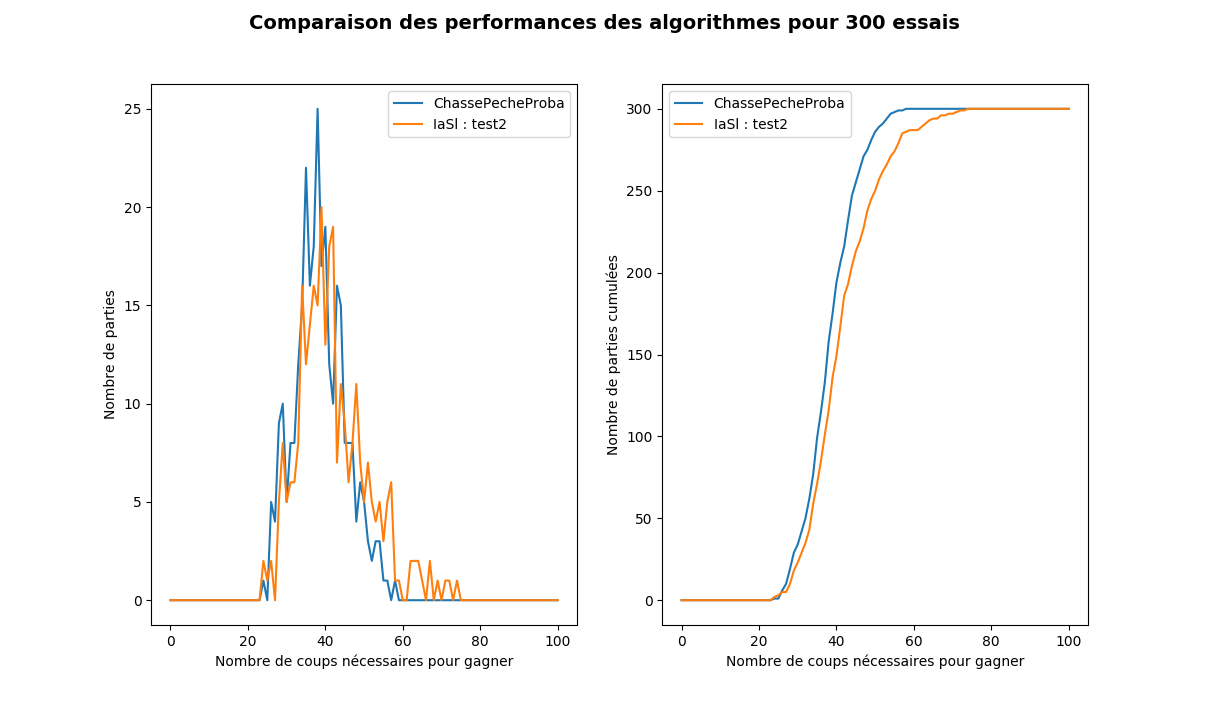
\includegraphics[width=.95\linewidth]{images/perfiasl3.png}
	        \caption*{Performance IA V2 (quelques heures d'entraînement)}
	        \label{fig:perfiasl3}
	    \end{figure}{}
	\end{frame}{}
	
	\begin{frame}{Amélioration et Entraînement}
	    \begin{figure}
	        \centering
	        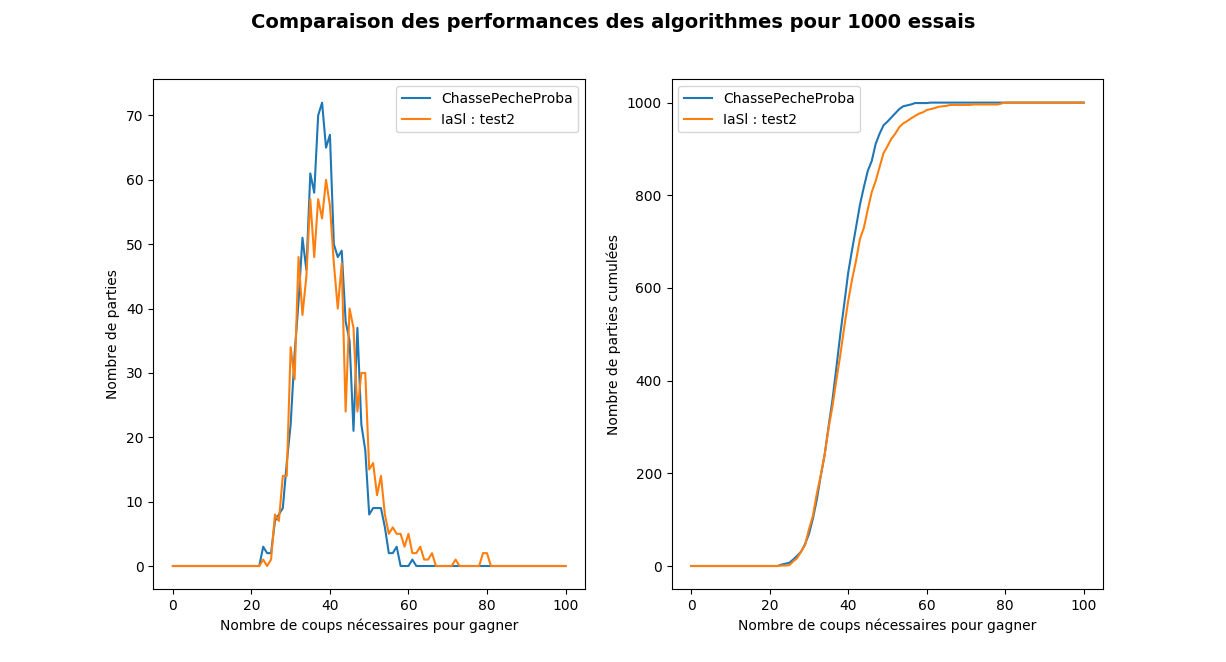
\includegraphics[width=.95\linewidth]{images/perfiasl4.png}
	        \caption*{Performance IA V2 (24h d'entraînement)}
	        \label{fig:perfiasl4}
	    \end{figure}{}
	\end{frame}{}

\subsection{Tensoflow}
	
	\begin{frame}{La librairie Tensorflow}
		\begin{block}{Avantages}
		    \begin{itemize}
		        \item Librairie libre, gratuite et open source
		        \item Primitives et écosystème pré-codés et prêts à l'emploi
		        \item Performances accrues car développée par des professionnels
		        \item Support et formations accessible car librairie très utilisé
		    \end{itemize}{}
		\end{block}
		\begin{minipage}[c]{0.68\linewidth}
		    \begin{block}{Inconvénients}
        	    \begin{itemize}
        	        \item Perte de contrôle et de ??? % TODO : compléter
        	        \item Formation obligatoire
        	        \item Initialement développé par Google
        	    \end{itemize}{}
		    \end{block}
        \end{minipage}
        \begin{minipage}[c]{0.30\linewidth}
            \centering
            
\includegraphics[height=1.5cm]{images/tflogo.png}
        \end{minipage}
	\end{frame}
	
	\begin{frame}{Performances après entraînement}
	    \begin{figure}
	        \centering
	        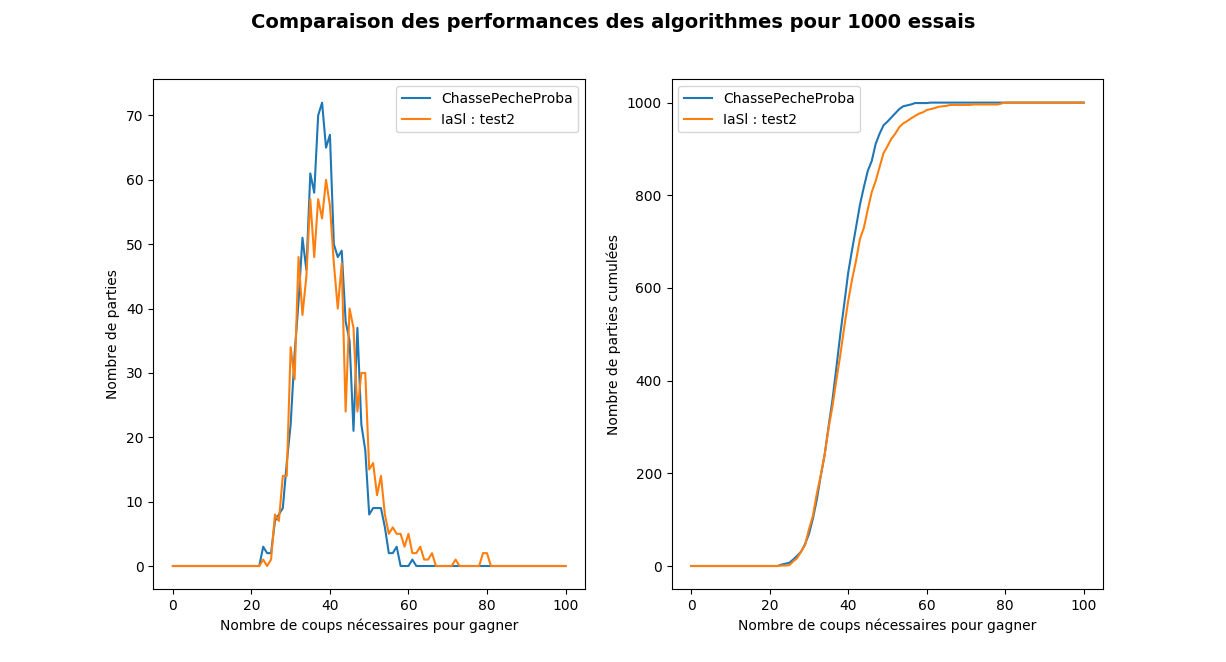
\includegraphics[width=.95\linewidth]{images/perfiasl4.png} % TODO : mettre le bon graphique
	        \caption*{A compléter}
	        \label{fig:perfstf}
	    \end{figure}{}
	\end{frame}{}

\subsection{Résultats}
	
	\begin{frame}{Comparaison des performances des différentes IA}
		\begin{figure}
	        \centering
	        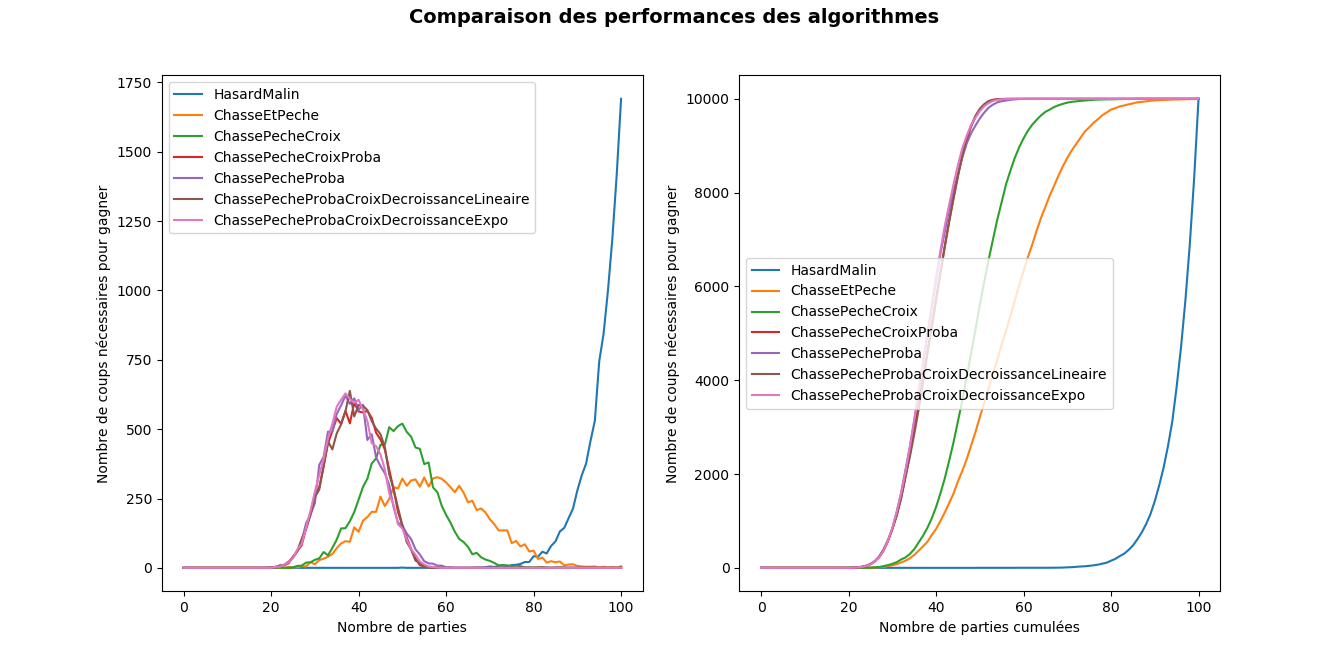
\includegraphics[width=.95\linewidth]{images/perfsstats.png} % TODO : mettre le bon graphique
	        \caption*{A compléter}
	        \label{fig:perfssl}
	    \end{figure}{}
	\end{frame}